\chapter{Global Event Reconstruction}\label{chap:emul}
\section{Particle Flow}
The Particle Flow algorithm is the all purpose method that is used to reconstruct events in the CMS detector of the Large Hadron Collider.
\subsection{PUPPI}
	
\section{Event and Jet Reconstruction}\label{eventsel}
In the CMS experiment, the Particle Flow (PF) algorithm \cite{particleflow} is used to reconstruct final state particles by linking information from the individual subdetectors to form a global event description. PF candidates are classified as either a muon, photon, charged hadron, or neutral hadron, ensuring that there is no double counting of of particles.
\subsection{Event Reweighting and Quality Checks}
Simulation may not accurately reflect the data due to high order effects or detector effects. To ensure that our simulation samples are representative of the data, final event counts in simulation are re-weighted to resemble the distributions observed in data. Additionally, we apply other quality checks that remove events not suitable for physics analyses due to imperfect detector conditions or poorly reconstructured variables.
\subsubsection{L1 Prefiring}\label{prefiring}
During the 2016 and 2017 data taking periods, the gradual timing shift of the ECAL was not properly propgated to the L1 trigger primitives (TP), resulting in an inefficiency for objects with $\eta > 2.0$. These high eta TPs were mistakenly associated with the previous bunch crossing; not only would this cause that trigger primitive to be missing from the correct bunch crossing, but it could cause events to self-veto if there is a significant amount ECAL energy in $2<|\eta|<3$ since L1 rules forbid two consecutive bunch crossings from firing. This effect is not described by simulations and must be accounted for by re-weighting our simulation samples. The weights are obtained by taking the product of the non-prefiring probability of all objects with overlap removal and are provided by the collaboration \cite{l1prefiring}.
\subsubsection{Primary Vertices}
Primary vertices are identified by clustering tracks based on the z-coordinate of their point of closest approach to the center of the beam spot. The clustering algorith must balance the ability to reolve nearby vertices in cases of high pileup against the possibility of splitting a single, genuine interaction vertex into more than one cluster. For this reason a deterministic annealing alogirthm is used in CMS \cite{trackPVCMS2014}. Each of the reconstructed primary vertices is then required to satisfy quality criteria: $\sqrt{x^2+y^2}<2$ cm, is not fake (i.e. is not a vertex made out of a proper fit to tracks), $\abs{z}<24$ cm, and $N_{dof} > 4$.  The primary vertex with the highest $\Sigma\pt^2$ is assigned as the leading primary vertex (PV). All other verticies are considered pileup (PU) vertices.
\subsubsection{Pileup Re-weighting}\label{PUSF}
To account for discrepancies between the pileup profile of the simulated samples and data, we apply pileup reweighting to the MC samples. The weights are determined from the ratio of the pileup distribution in data and in MC, with both distributions normalized to a unit area. The derived weights are provided by the CMS LUMI POG \cite{PUSFgithub} and are derived assuming using the full Run 2 cross-section of $\sigma_{MB}=69.2$ mb. There is a $\pm 4.6\% $ uncertainty \cite{LUMIPOGtwiki} on this cross-section measurment, and that is propagated to the weight uncertainties by scaling the cross-section up and down by this value and re-deriving the weights.
\subsubsection{2018 HEM issue}
During 2018 data-taking two HCAL modules' power supplies died, impacting the jet energy measurement in this region \cite{HEM}. In order to account for this issue we reject the event if any jet
 in the $-1.57 < \phi < -0.87$ and $-3.0 < \eta < -1.3$ region for the 2018 dataset.
\subsection{Jets}\label{jets}
Jets are reconstructed by clustering all charged PF candidates reconstructed from the primary vertex and all other neutral PF candidates. Due to its resilience against soft radiation, the anti-$k_T$ \cite{antikt} algorithm is used as the cluster jets in CMS. For this analysis that is considering the high \pt or boosted regime, we use AK8 jets, or jet's clustered using anti-$k_T$ and a radius of $R=0.8$. The pileup per particule identification (PUPPI) \cite{puppi} algorithm is use to mitgate pileup in these jets.\\
To suppress identifying jets originating from detector noise, miscalibration of detector components, or misreconstructed objets, the tight jet ID requirement \cite{jetid}. Distributions of $\eta-\phi$ for each era are shown in \ref{fig:jetvetomap} and are sufficiently flat after selections, needing no further correction or veto beyond the 2018 HEM veto.

\begin{figure}[h!]
  \centering
  \begin{subfigure}
      \centering
  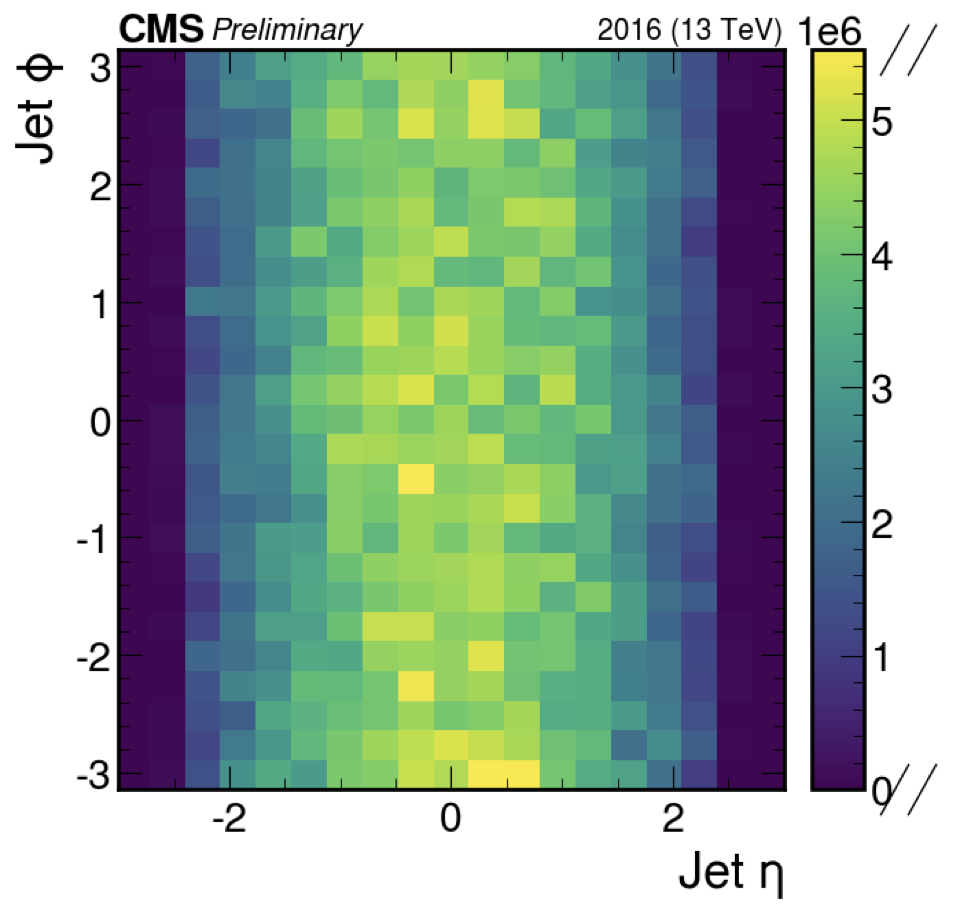
\includegraphics[width=.23\linewidth]{figures/multijet/dijet/eta_phi_2016.png}
    \end{subfigure}
    \begin{subfigure}
      \centering
      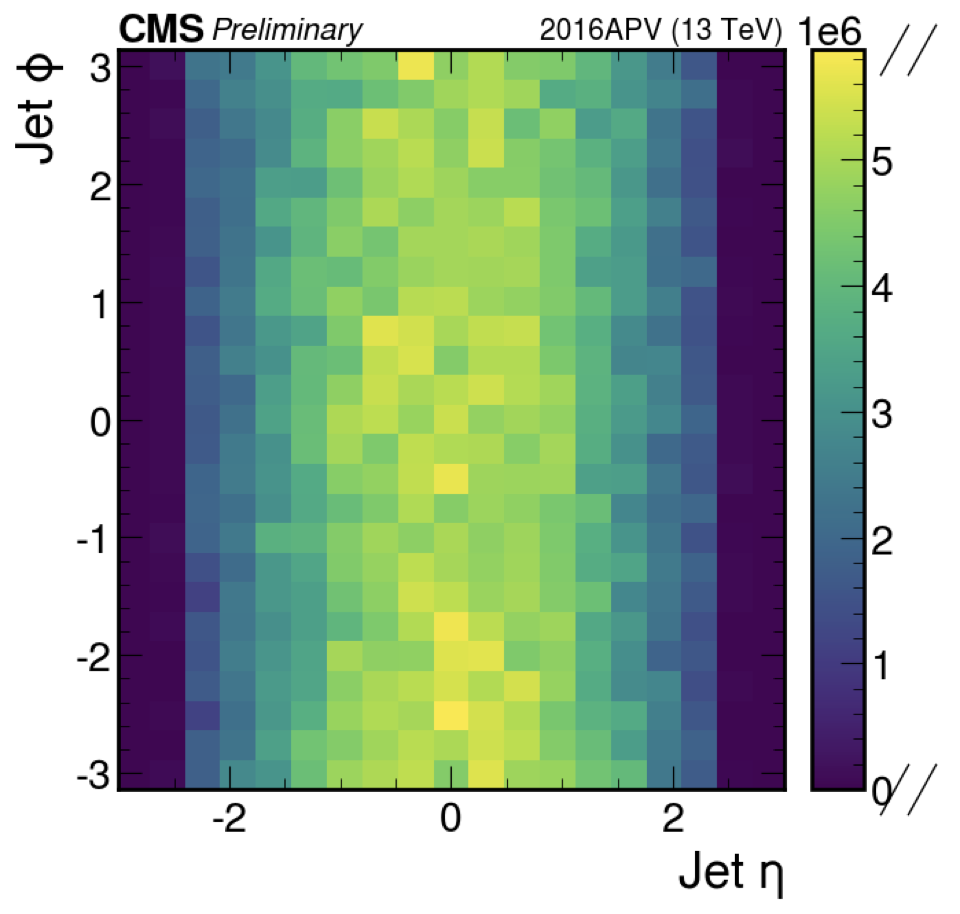
\includegraphics[width=.23\linewidth]{figures/multijet/dijet/eta_phi_2016APV.png}
    \end{subfigure}
    \begin{subfigure}
      \centering
      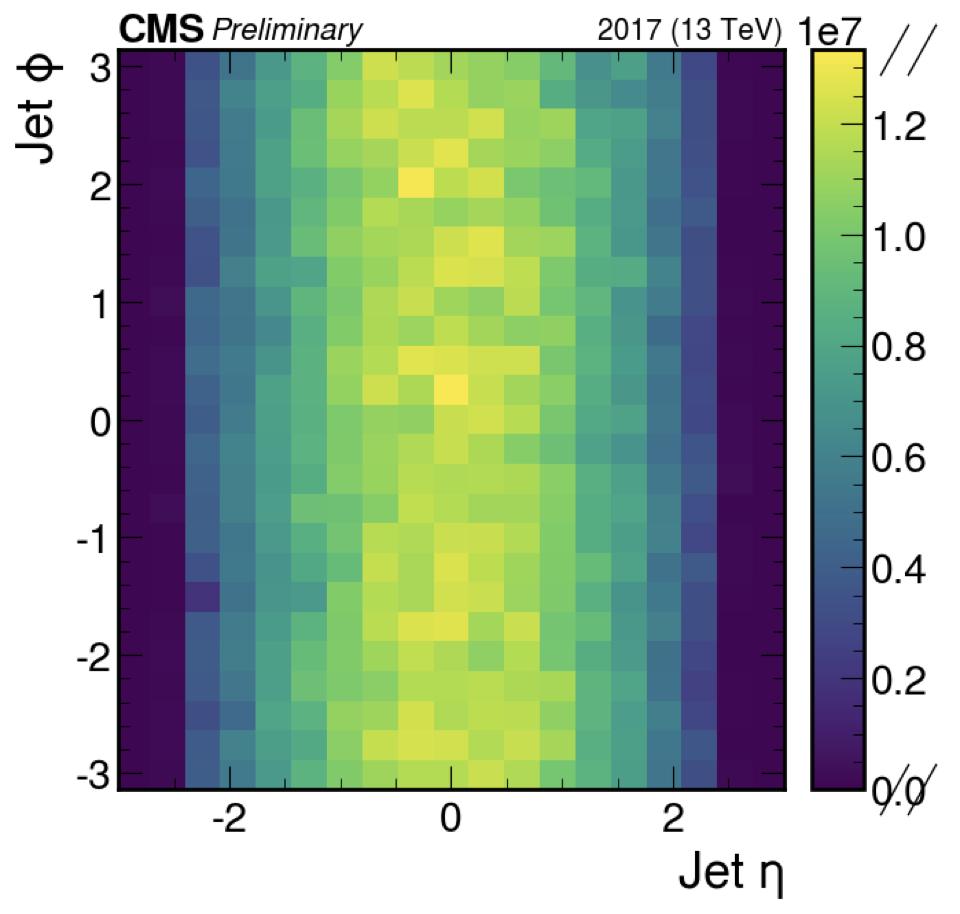
\includegraphics[width=.23\linewidth]{figures/multijet/dijet/eta_phi_2017.png}
    \end{subfigure}
    \begin{subfigure}
      \centering
      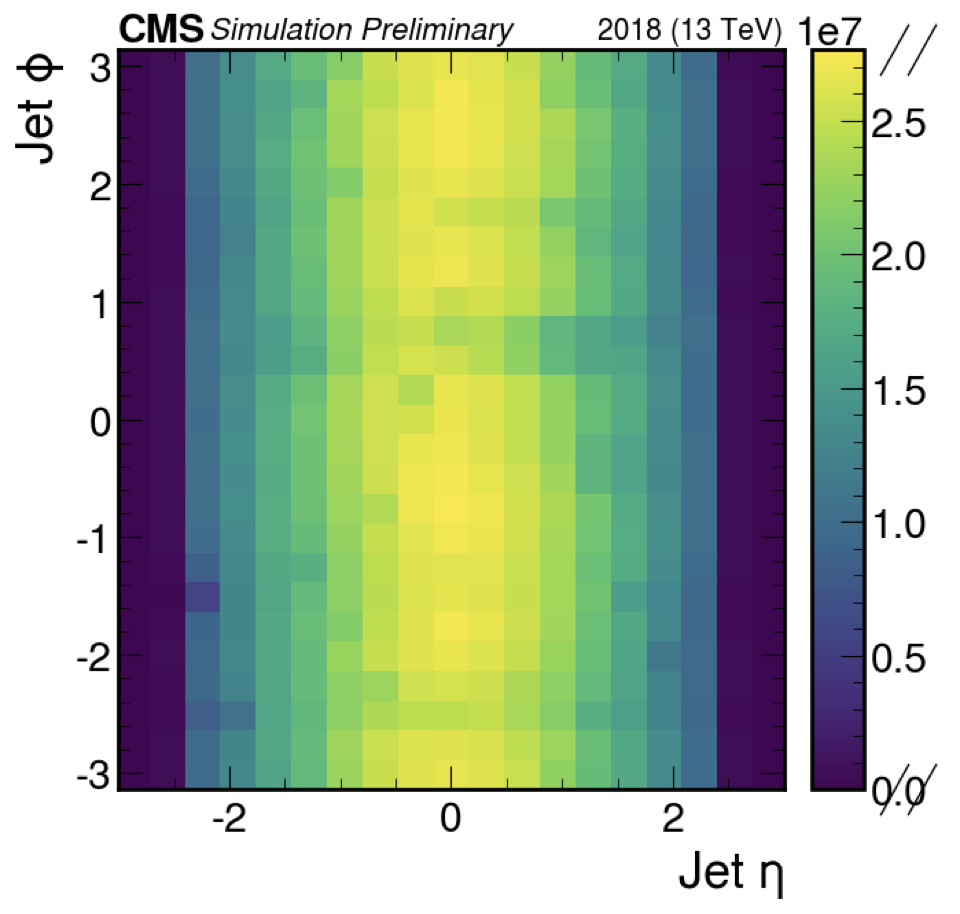
\includegraphics[width=.23\linewidth]{figures/multijet/dijet/eta_phi_2018.png}
    \end{subfigure}
    \caption{$\phi$ vs. $\eta$ distribution for each era of data taking. All are sufficiently flat to not require further veto maps, except 2018 which required the HEM veto.}
    \label{fig:jetvetomap}
\end{figure}
  
\subsubsection{Jet Energy Corrections}\label{JEC}
Kinematic observables and the reconstruction and selection efficiencies between the reconstruction of data and simulation do not agree exactly. This is to be expected since simulation is an approximation of the real world image, but to produce a reliable measurement we calibrate the jet energu and momenta to improve the agreement between data and simulation. Changing the measured value of the jets also affects the event yield after selections, so the yield in simulation is corrected to be the same as that of the data. The jet energy scales in simulation are corrected for pileup (PU) effects and differences in the momenta between data and simulation. Jets in data are additionally corrected for residual detector and reconstruction affects. The factors for the correction of the jets' momenta in data and simulation and their uncertainties are provided by the CMS collarboration as a function of \pt and $\eta$.\\
The jet \pt resolution is relatively poor compared to other physics objects; to prevent a bias from the smearing of this resolution, after JES corrections are applied, the reconstructed jet momenta is scaled so that the resolution matches that of the simulation at the particle level. For a reconstructed jet matched to a jet at the generator level, it's momentum is scaled by the factor:
\begin{equation}
  \label{eq:JER}
  c_{\textrm{JER}}=1+(s_{\textrm{JER}}-1)\frac{\pt^{\textrm{RECO}}-\pt^{\textrm{GEN}}}{\pt^{\textrm{RECO}}}
\end{equation}
The resolution scale factor $\sigma_{\textrm{JER}}$ and their corresponding uncertainties are provided by the CMS collaboration.
%Describe how JECs are applied to subjets adn softdrop mass is reconstructed from that
% Don't need PU jet id bc it's only applied to jets w/ pt below 50 GeV
% TODO: do  i need muon suppression too? or only Z+jet
% TODO : do i need MET filters?
\subsubsection{Jet Mass}
The main observables for this analysis are jet mass and \pt. The invariant jet mass is defined as
\begin{equation}
m_{j}^2 = P_\mu P^\mu  = \left(\Sigma_{i\in jet}p_i^2\right)
\end{equation}
where $P_\mu$ is the totoal four-momentum of the jet, constructed by summing the four momenta $p_i$ of all the consituents of the jet. To the first non-trivial order (NLO), for a jet originating from a massless parton, the invariant mass is:
\begin{equation}
\langle M^2\rangle  \simeq C\frac{\alpha_s}{\pi}p_T^2R^2
\end{equation}
where $C$ depends on the fraction of quarks and gluons in the jet and type of jet algorithm used \cite{jetography}. Perturbative effects from parton splitting in the soft and collinear limits and non-perturbative effects from hadronisation and underlying event are limiting factors when performing calculations of the jet mass.
% TODO: add more details about jet mass resummaton and sudakov form factors, etc... in the context of individual splittings
\subsubsection{Soft Drop Mass}
To mitigate effects from underlying event radiation, initial state radiation, and pileup, jets can be treated with grooming techniques, which aim to remove wide-angle soft  radiation from jets. CMS utilizes the soft drop algorithm \cite{softdrop} to groom jets and derive jet substructure variables such as the soft drop groomed jet mass $m_{SD}$. The soft drop algrotithm is a generalization of the modified Mass Drop Tagger (mMDT) procedure \cite{mMDT}. To perform soft drop grooming, the jets are reclustered using the Cambridge-Achen (CA) \cite{CA} clustering algorithm, and then steps backwards through it's clustering history. At each step, the two resulting subjets are compared and the softer subjet is removed until the soft drop condition is satisfied:
\begin{equation}
\frac{\min(p_{T1},p_{T2})}{p_{T1}+p_{T2}}>z_{cut}\left(\frac{\Delta R_{12}}{R_0}\right)^\beta
\end{equation}
where $p_{Ti}$ are the tranvserse momenta of the subjets w.r.t beam, $\Delta R_{12}$ is the distance between the subjets in the $\eta-\phi$ plane, $z_{cut}$ is the soft drop threshold, and $\beta$ is the angular exponent. $z_{cut}$ controls how aggressive the grooming is w.r.t \pt fraction, and in CMS is set to 0.1. The angular splitting $\beta$ reduces to the ungroomed jet when $\beta\rightarrow\infty$ and the lower the value of $\beta$, the more collinear radiation is groomed away; CMS uses a value of $\beta=0$ which reduces the procedure to mMDT and vetoes both soft and soft-collinear radiation. While the soft drop jet mass ($m_{SD}$) is IRC safe, the soft drop \pt is not IRC safe, but only Sudakov safe \cite{advancesInJet}; hence, we only use the soft drop mass as an observable along with the regular jet mass and \pt, but not the soft dropped \pt in this measurement.
% most likely will remove following section
\subsubsection{Jet Mass Scale and Resolution}\label{JMS} Just like the jet energy and momentum, the jet mass, especially for boosted jets (AK8 jets) and measurements using the softdrop mass, required corrections for a reliable comparison between data and simulated events. Jet mass scale and resolution scale factors are derived from a fit to the W-jet mass in data and simulation. These values are listed in table \ref{table:JMS} and provided by the collaboration.
\begin{table}[h!]
  \centering
\begin{tabular}{lllll}
\hline
\textbf{Year} & \textbf{JMS SF} & \textbf{JMS Unc.}         & \textbf{JMR SF} & \textbf{JMR Unc.}        \\ \hline
2016          & 1.00            &$\pm$ 0.0094 & 1.0             & $\pm$ 0.2   \\
2017          & 0.982           & $\pm$ 0.04   & 1.09            & $\pm$ 0.05  \\
2018          & 0.999           & $\pm$ 0.002  & 1.108           & $\pm$ 0.034 \\ \hline
\end{tabular}
  \caption{Jet mass scale and resolution factors and uncertainties for each era.}
  \label{table:JMS}
\end{table}
